\documentclass{beamer}

\usepackage[utf8]{inputenc}%           gestion des accents (source)
\usepackage[T1]{fontenc}%              gestion des accents (PDF)
\usepackage[francais]{babel}%          gestion du français
\usepackage{textcomp}%                 caractères additionnels
\usepackage{mathtools,  amssymb, amsthm}% packages de l'AMS + mathtools
\usepackage{lmodern}%                  police de caractère
\usepackage{geometry}%                 gestion des marges
\usepackage{graphicx}%                 gestion des images
\usepackage{xcolor}%                   gestion des couleurs
\usepackage{array}%                    gestion améliorée des tableaux
\usepackage{calc}%                     syntaxe naturelle pour les calculs
\usepackage[framemethod=TikZ]{mdframed}% print frames
\usepackage[justification=centering]{caption}%                  for captionof
\usepackage{listings}%				  pour insertion de codes 
\usepackage{enumitem}%                 pour les listes numérotées
\usepackage{microtype}%                améliorations typographiques
\usepackage{csvsimple}%                convertir un fichier .csv en tableau
\usepackage{url}%					  amélioration afficahge url
\usepackage{hyperref}%                 gestion des hyperliens
\usepackage{svg}	%					  gestion des svg	
\usepackage{float}%					  gestion des figure non flotante
 
\lstset{language=c++}
\definecolor{codegreen}{rgb}{0,0.6,0}
\definecolor{codegray}{rgb}{0.5,0.5,0.5}
\definecolor{codepurple}{rgb}{0.58,0,0.82}
\definecolor{backcolour}{rgb}{0.95,0.95,0.92}
 
\lstdefinestyle{mystyle}{
    backgroundcolor=\color{backcolour},   
    commentstyle=\color{codegreen},
    keywordstyle=\color{magenta},
    numberstyle=\tiny\color{codegray},
    stringstyle=\color{codepurple},
    basicstyle=\footnotesize,
    breakatwhitespace=false,         
    breaklines=true,                 
    captionpos=b,                    
    keepspaces=true,                 
    numbers=left,                    
    numbersep=5pt,
    otherkeywords={uint16_t},                  
    showspaces=false,                
    showstringspaces=false,
    inputencoding=latin1,
    showtabs=false,                  
    tabsize=2
}
\lstset{style=mystyle}

\hypersetup{%
    pdfborder = {0 0 0}
}

\usetheme{Luebeck}
\addtobeamertemplate{footline}{\hfill\insertframenumber/\inserttotalframenumber\hspace{2em}\null}

\usenavigationsymbolstemplate{}

\setbeamersize{text margin left=10px}
\setbeamersize{text margin right=10px}


\title{Projet PSAR}
\subtitle{Dispositif Autonome de Synthèse Sonore}
\institute{Encadrant : Hugues Genevois}
\author{Pierre Mahé}
\date{\today}

\titlegraphic{
	
\includegraphics[height=30px]{upmc_logo.jpg}	
	\hspace{4cm}
	
\includegraphics[height=30px]{LogoLAM.jpg}}
\begin{document}

\begin{frame}
\titlepage
\end{frame}
\begin{frame}
\frametitle{Le Dispositif}
\begin{figure}
  \centering
  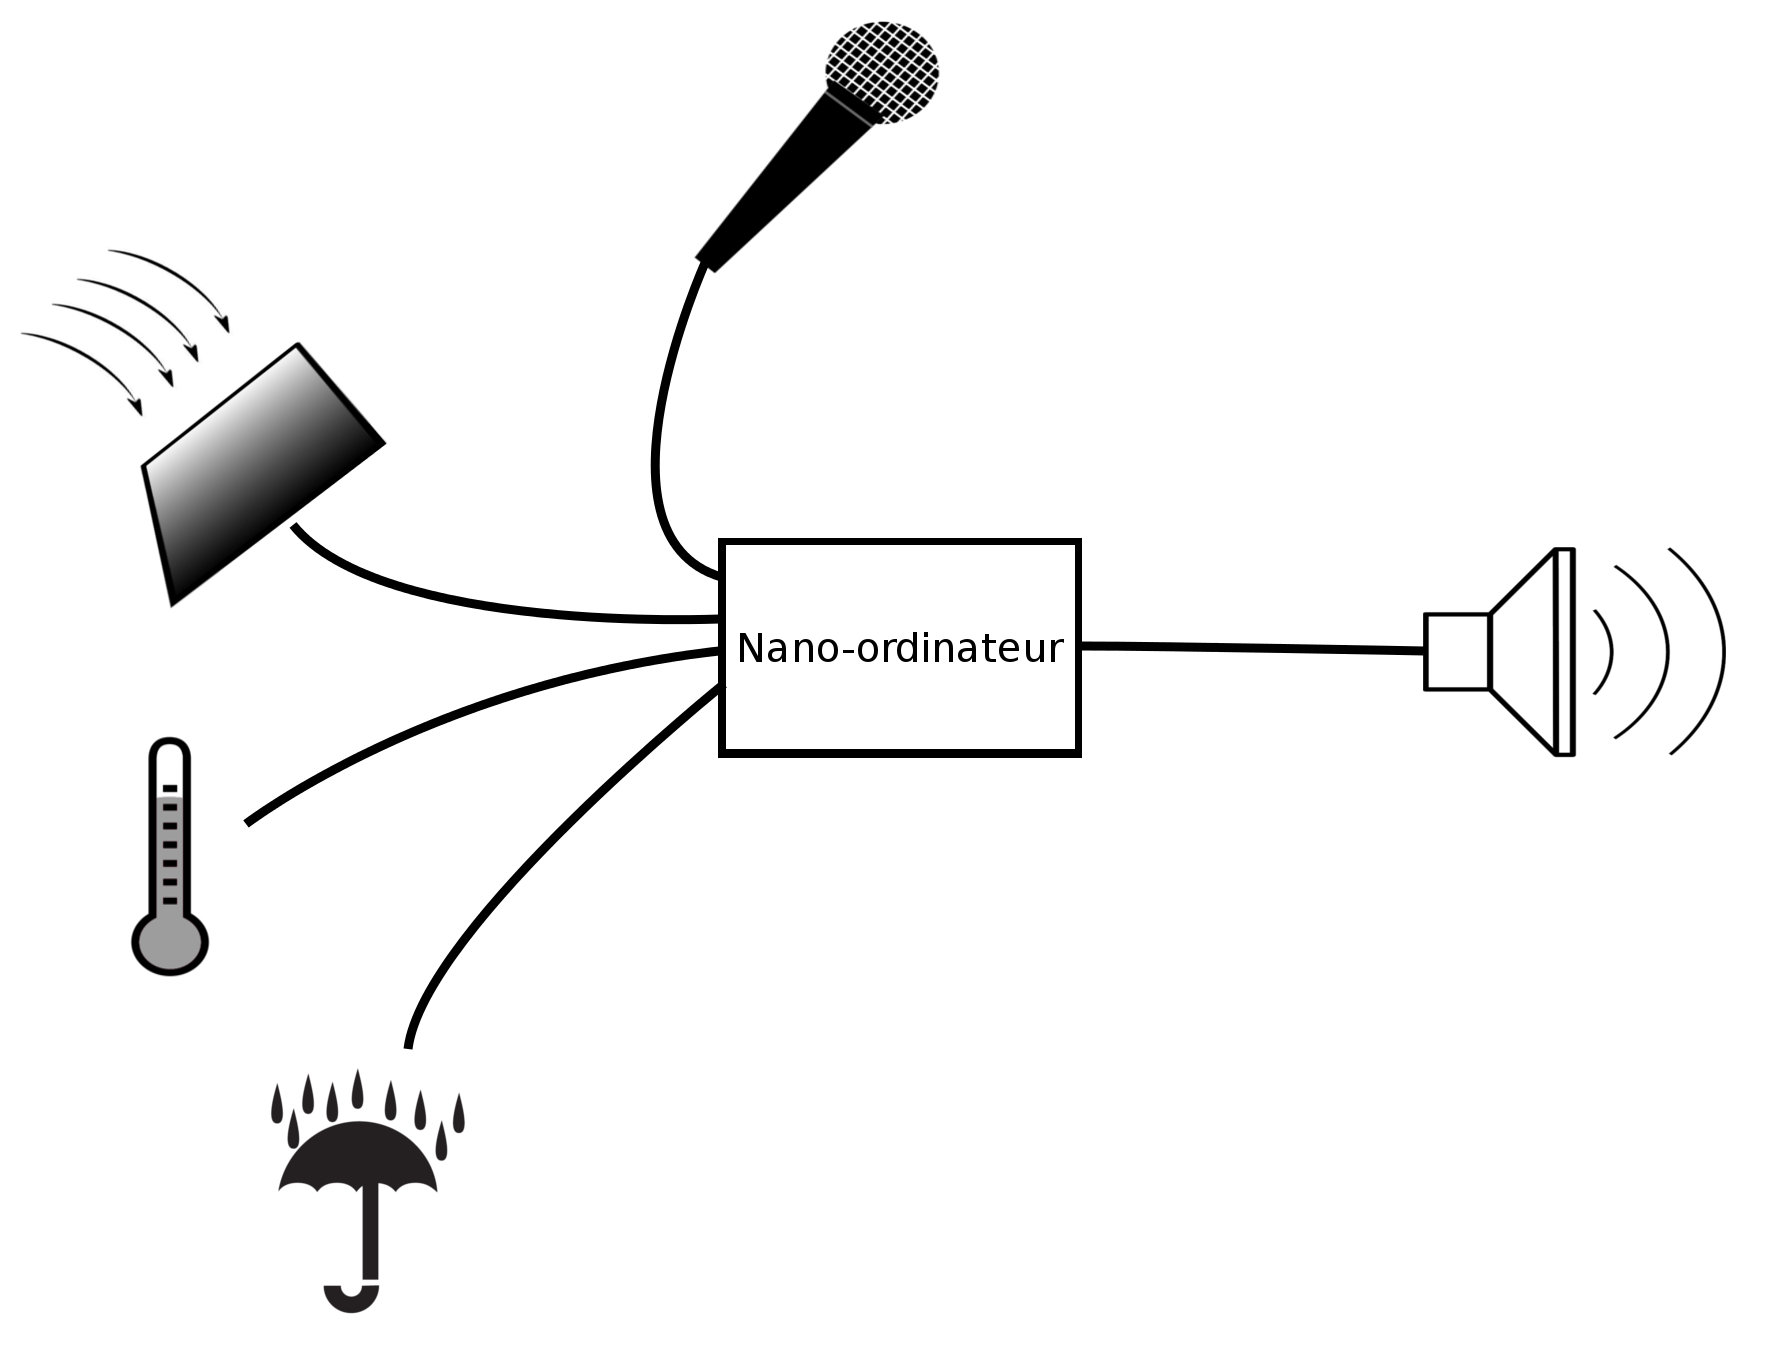
\includegraphics[height=200px]{schemagrobal.jpg} 
	\caption{Le Dispositif}
	
\end{figure}\end{frame}

\begin{frame}
\frametitle{Contraintes du projet}
\framesubtitle{La Carte Udoo}
\begin{minipage}{0.49\textwidth}
\textbf{Avantages:}
\begin{itemize}
\item Compatibilité Arduino
\item Bonne plate-forme d’expérimentation
\item Distribution Linux
\item Prix raisonnable
\end{itemize}
\end{minipage}
\begin{minipage}{0.49\textwidth}
\begin{figure}
  \centering
  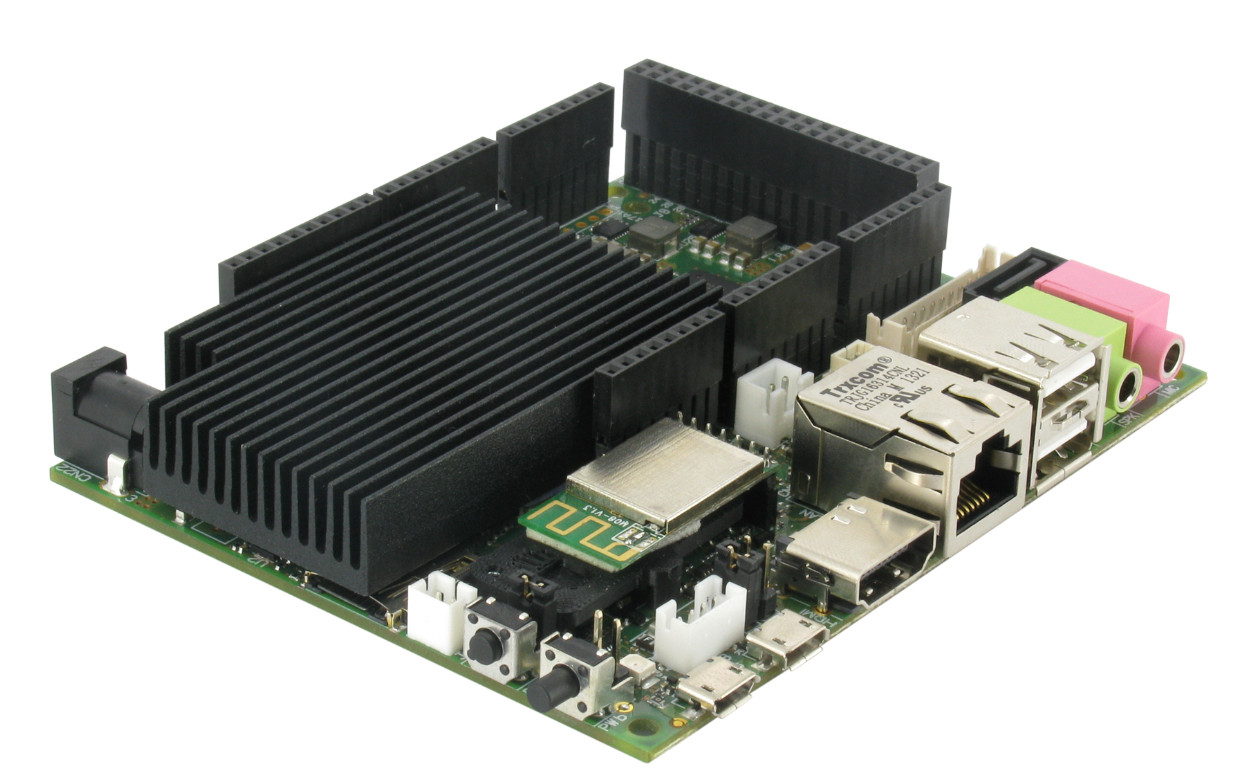
\includegraphics[width=\textwidth]{udoo.jpg} 
	\caption{Carte Udoo}
\end{figure}
\end{minipage}
\end{frame}

\begin{frame}
\frametitle{Contraintes du projet}
\framesubtitle{Pure Data}
\textbf{Pure Data}
\begin{itemize}
\item Langage Graphique pour la création et l'interaction musical temps réel.
\item Définir des modules appelés \texttt{boîtes}.
\item Créer des modules en \texttt{C++} appelé \texttt{External}.
\item Modifier les patchs durant l’exécution du programme.
\item De nombreuse fonctionnalités sont déjà implémentés.
\end{itemize}
\end{frame}

\begin{frame}
\frametitle{Contraintes du projet}
\framesubtitle{Pure Data}
\textbf{Exemple de Patch}
\begin{figure}
  \centering
  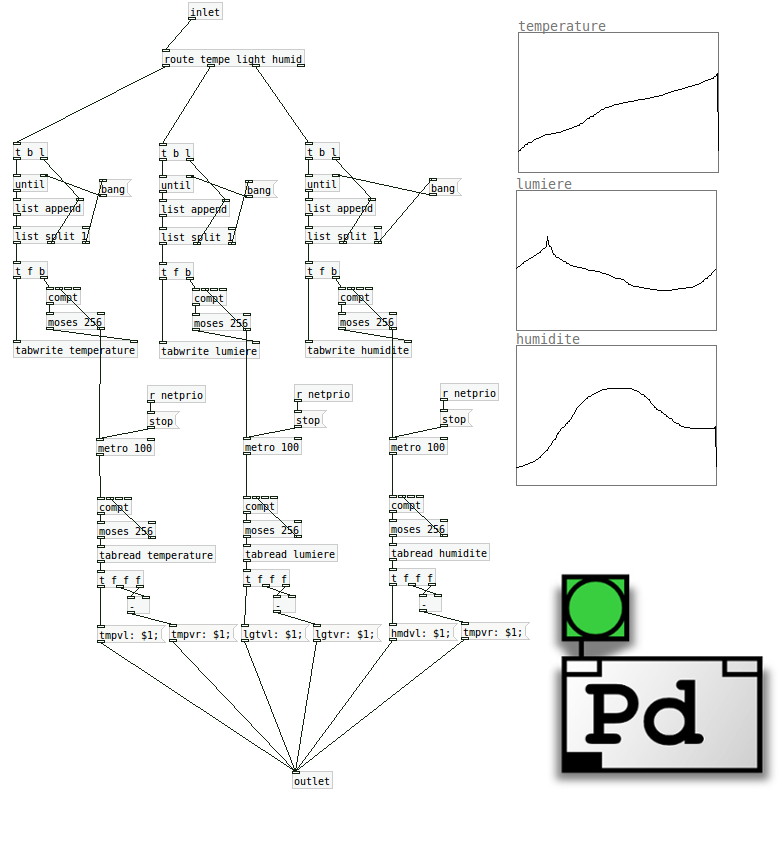
\includegraphics[width=160px]{pd.jpg} 
	\caption{Patch Pd}
\end{figure}
\end{frame}

\begin{frame}
\frametitle{Structure du projet}
\begin{figure}
  \centering
  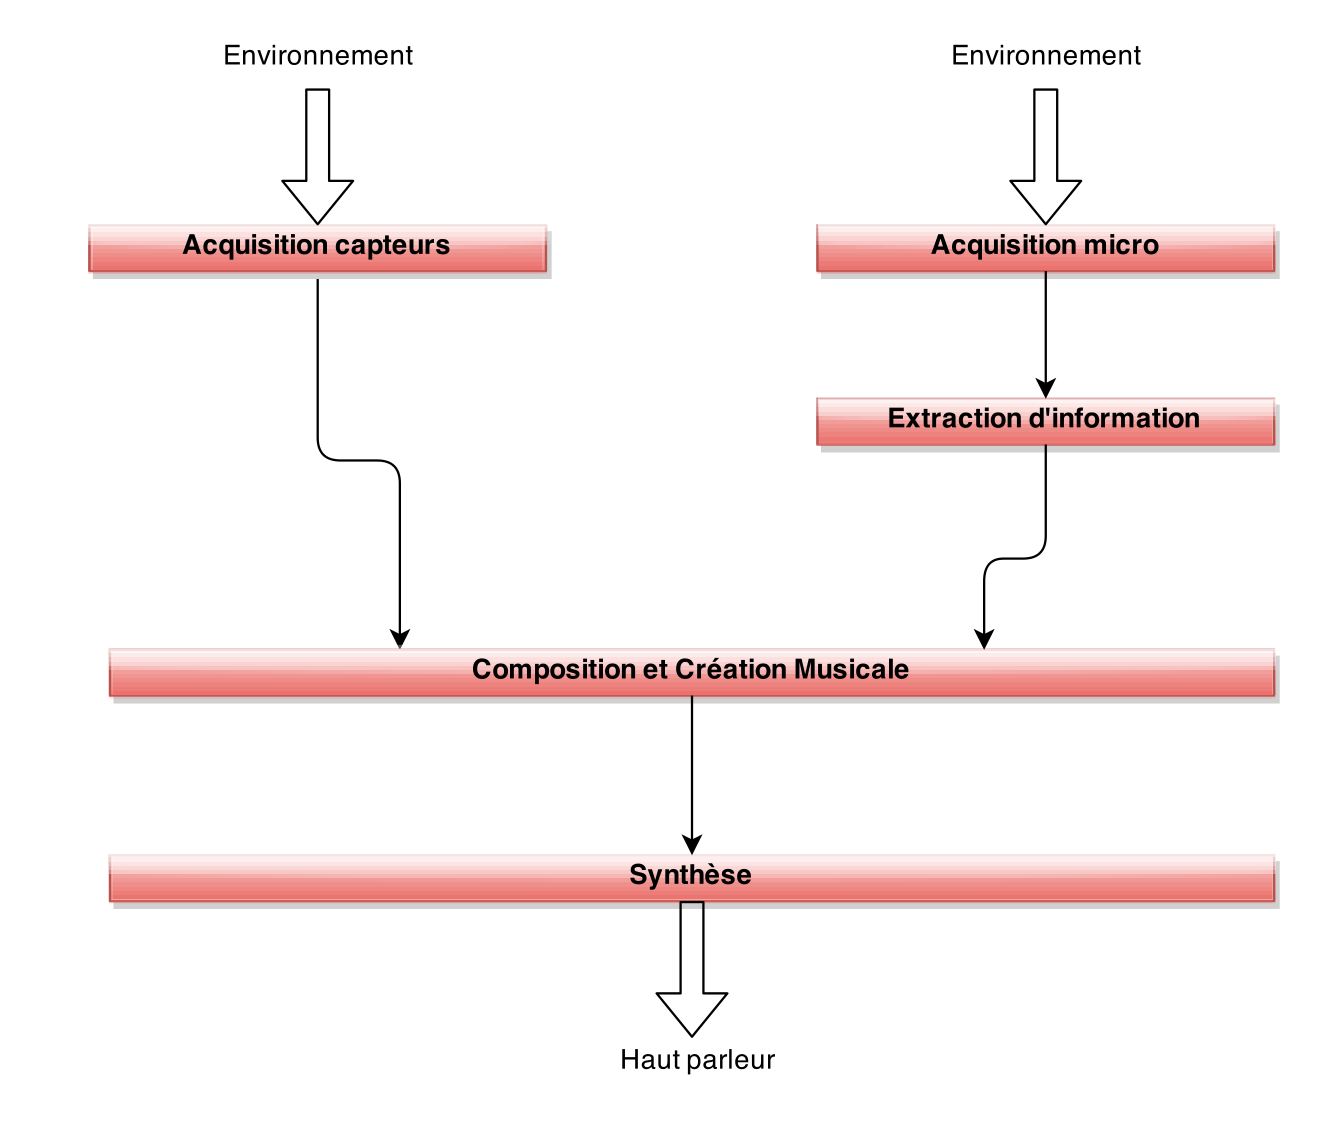
\includegraphics[height=225px]{structprojet.jpg} 
\end{figure}
\end{frame}


\begin{frame}
\frametitle{Récupération de l'environnement}
\begin{figure}
  \centering
  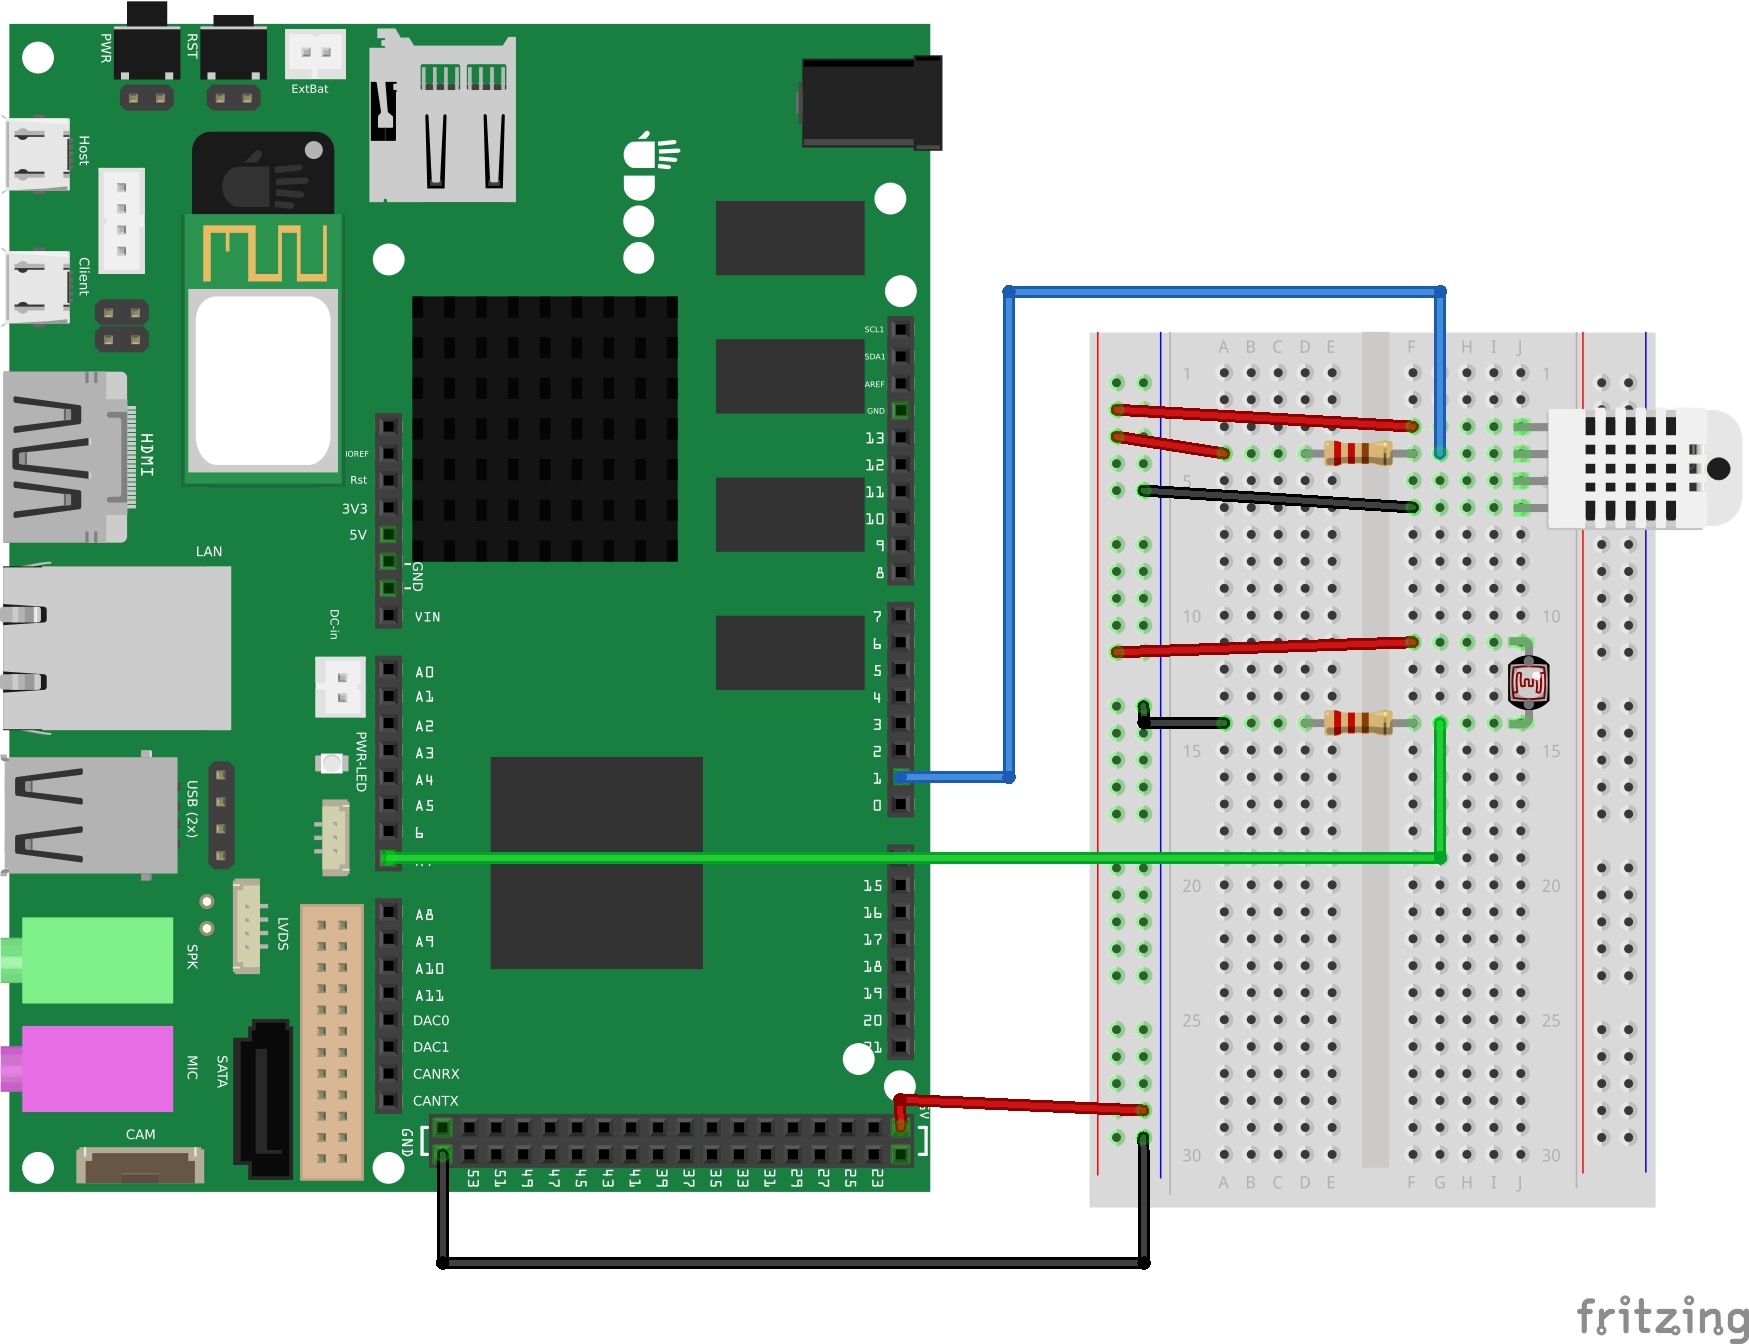
\includegraphics[width=150px]{montage.jpg}  
  \hspace{15px}
  \includegraphics[width=150px]{montagephoto.jpg} 
	\caption{Montage sur la carte Udoo}
\end{figure}
\begin{figure}
\centering
\vspace{-0.5cm}
\includegraphics[height=30px]{protocole.jpg}
\caption{Messages échangés entre la partie Arduino et Pure Data}
\end{figure}
\end{frame}

\begin{frame}
\frametitle{Traitement audio}
\framesubtitle{Mélodie}
Partage du spectre sonore en plusieurs bandes de fréquences à l'aide de filtres.\\
Détection de la fréquence principale de chaque bande.
\begin{figure}
\centering
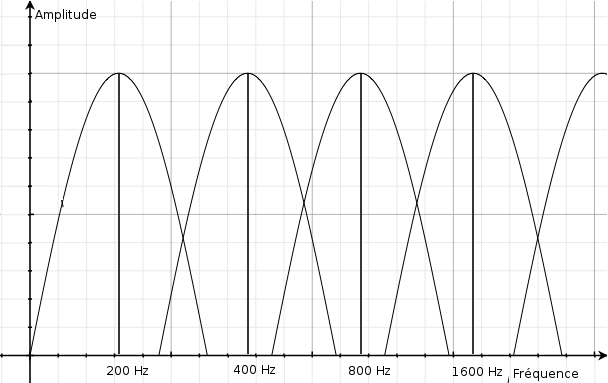
\includegraphics[height=100px]{filtre.jpg}
\caption{Filtrage par bandes de fréquences}
\end{figure}
Pour limiter les fausses détections, des \texttt{Noise Gates} suppriment les signaux parasites.
\end{frame}


\begin{frame}
\frametitle{Traitement audio}
\framesubtitle{Mélodie}
\textbf{Ce module permet de récupérer deux informations utiles}
\newline
\newline
\textbf{Un compteur de notes}, fournissant périodiquement la fréquence d'apparition de chaque note.
\newline
\newline
\textbf{La mesure de la répartition des fréquences}\\
Pour ne pas perdre la hauteur du son capté par le micro.
\end{frame}


\begin{frame}
\frametitle{Traitement audio}
\framesubtitle{Rythme}
Pour que le dispositif joue des sons cohérents avec l’environnement, le dispositif extrait également le rythme.\\
Création d'un module pour détecter les débuts de notes à l'aide d'une boite détectant les impacts dans un signal.

\begin{figure}
\centering
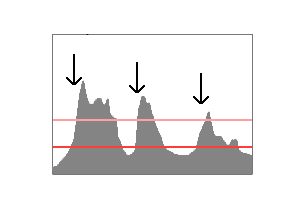
\includegraphics[height=130px]{bonk.jpg}
\caption{Fonctionnement de \texttt{bonk}}
\end{figure}
\end{frame}

\begin{frame}
\frametitle{Traitement audio}
\framesubtitle{Rythme}
Les rythmes détectés sont groupés en séquence.\\
Le module procède à une normalisation de la durée des rythmes.
\begin{figure}
\centering
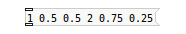
\includegraphics[height=20px]{rythme.jpg}
\caption{Séquence rythmique détectée}
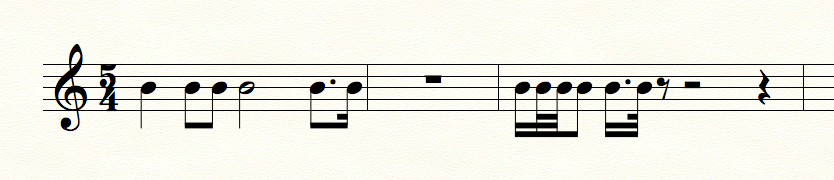
\includegraphics[height=50px]{structurerythme.jpg}
\caption{Séquence rythmique pouvant produire la séquence}
\end{figure}
\end{frame}

\begin{frame}
\frametitle{Traitement audio}
\framesubtitle{Rythme}
Un External se charge de détecter des motifs récurrents dans la séquence.\\
Dès qu'une séquence est trouvée, l'external retourne ce motif.\\
La taille du motif est paramétrable.
\begin{figure}
\centering
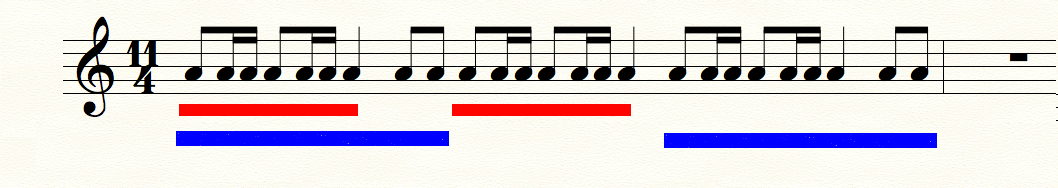
\includegraphics[height=50px]{motifrythme.jpg}
\caption{Motif rythmique}
\end{figure}
\end{frame}


\begin{frame}
\frametitle{Interface Utilisateur}
\begin{minipage}{0.49\textwidth}
\textbf{Permet à l'utilisateur}\\\\
L'envoi de données pour simuler les capteurs.\\\\
Changement du module de Création Musicale
\end{minipage}
\begin{minipage}{0.49\textwidth}
\begin{figure}
  \centering
  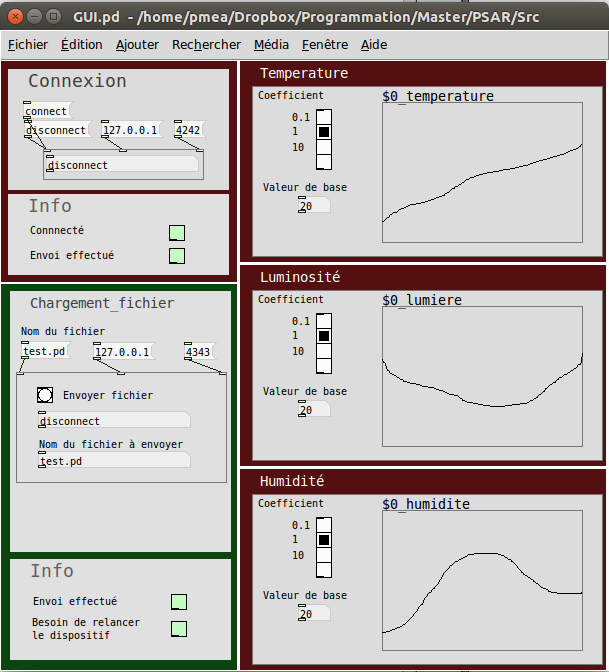
\includegraphics[width=\textwidth]{GUI.jpg} 
	\caption{Interface utilisateur}
\end{figure}
\end{minipage}
\end{frame}


\begin{frame}
\frametitle{Pour aller plus loin}
\textbf{Tests en environnement réel}\\
Il est difficile de couvrir toutes les configurations possibles.\\
Des tests supplémentaires en environnement réel auraient été souhaitables.
\newline
\newline
\textbf{Tests énergétique}\\
La carte Udoo étant très énergivore, il serait intéressant d'installer le dispositif sur d'autre carte plus économe en énergie.
\newline
\newline
\textbf{Serveur distant}\\
Il serait intéressant de réfléchir à une version utilisant un serveur.
\end{frame}

\end{document}